\documentclass[12pt,a4paper]{article}

\usepackage{float}
\restylefloat{figure}
\usepackage{hyperref}
\usepackage{graphicx}
\usepackage{gensymb}
\usepackage[title]{appendix}
\usepackage[dotinlabels]{titletoc}
\usepackage[nottoc,numbib]{tocbibind}
\usepackage{mathtools}
\usepackage[margin=0.5in]{geometry}
\renewcommand{\thefootnote}{\arabic{footnote}}

\newcommand*\wrapletters[1]{\wr@pletters#1\@nil}
\def\wr@pletters#1#2\@nil{#1\allowbreak\if&#2&\else\wr@pletters#2\@nil\fi}

\usepackage{enumitem}
\setenumerate{itemsep=0pt}

% Add support for multi-page tables.
\usepackage{longtable}

\pagenumbering{arabic}

\title{EE4DSA Coursework 1}
\author{Chris Cummins}

\begin{document}
\maketitle

\section{Disassembling the program ROM}

The file \texttt{rom.asm} contains a heavily annotated disassembled
version of the safe unlocking program, using the six instruction
mnemonics and a standard assembly syntax. The program tests for the
safe code 0702.

The assembly code was generated automatically using a disassembler
developed for this purpose, available at
\url{http://chriscummins.cc/disassembler}. The purpose of the
disassembler is to take as input a sequence of instructions, and to
generate an annotated explanation of the purpose of each
instruction. For example:

\begin{figure}[H]
  \centering
  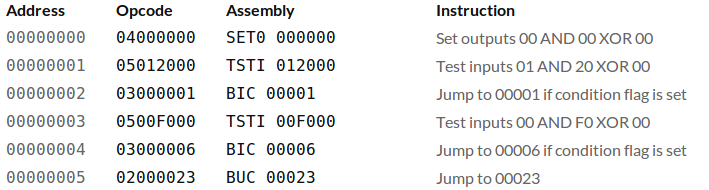
\includegraphics[width=5in]{assets/disassembled.png}
\end{figure}

Two further extensions to this disassembler were made. The first was
to provide a visualisation of program flow, in the form of a flow
chart. For example:

\begin{figure}[H]
  \centering
  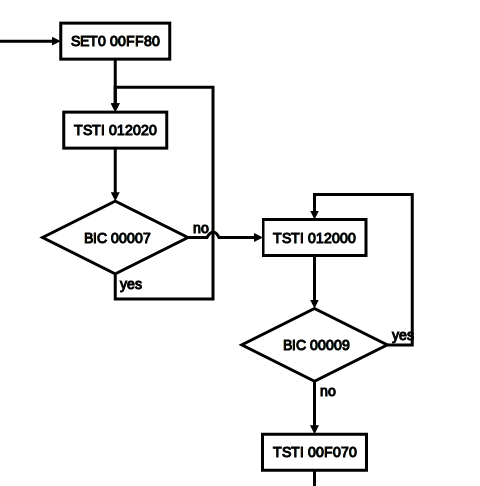
\includegraphics[width=3.5in]{assets/chart.png}
\end{figure}

The key to implementing this visualiser was to treat each instruction
within a program as a node in a data set. Each node can have multiple
children that it points to. In the case of an unconditional
instruction, there is a single child node (the next
instruction). Conditional instructions have two children nodes: the
next instruction, and the instruction to jump to if the condition is
met. In this manner, the set of nodes can be visualised as a tree, and
a simple third party library is used to generate the flow
chart. Future development could include adding a more complex
visualisation front-end to allow for more aesthetically pleasing chart
layouts, or to allow the user to arrange the chart components
themselves.

The second addition to the disassembler was the ability to generate
convincing assembler code. This involved adding the ability to create
symbolic links between instruction nodes, so that instructions could
be referenced by symbolic labels rather than by absolute
addresses. This has the benefit of making program flow a lot easier to
read, for example:

\begin{figure}[H]
  \centering
  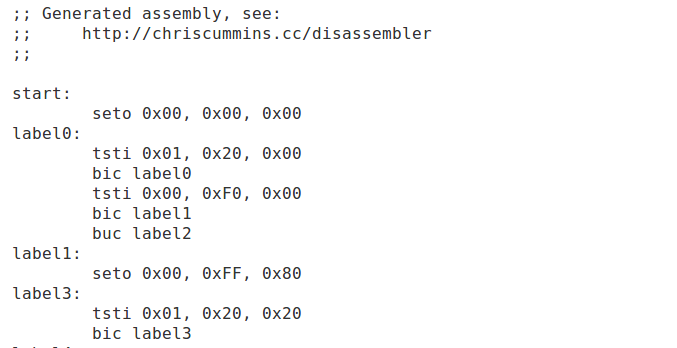
\includegraphics[width=6in]{assets/assembly.png}
\end{figure}

The disassembler is
implemented in JavaScript, with the source code available at\\*
\url{http://chriscummins.cc/js/disassembler.js}.

\section{Modifying the ROM program}

The file \texttt{rom.dat} contains a modified ROM program which uses
the last four digits of my SUN number (5189) as the code to the
safe. The only modifications required were to the \texttt{AND}
components of the four \texttt{TSTI} instructions. The
\texttt{test\_bench\_inputs.dat} file was then modified so as to test
this new code, and a process was added to the test bench program which
created a new \texttt{test\_bench\_outputs.dat} file.

\newpage
\begin{verbatim}
    process
      file     data_file: text;
      variable data_line: line;
    begin

      file_open(data_file, "my_test_bench_outputs.dat", write_mode);
      wait for 4500 ns; -- Halfway into first clock cycle

      while end_flag = '0' loop
        write(data_line, std_logic_vector(test_pc));
        write(data_line, ' ');
        write(data_line, test_opcode);
        write(data_line, ' ');
        write(data_line, test_ins_data);
        write(data_line, ' ');
        write(data_line, ld);
        write(data_line, ' ');
        write(data_line, now);

        writeline(data_file, data_line);
        wait for clk_period;
      end loop;

      file_close(data_file);
      wait;

    end process;
\end{verbatim}

\section{Implementing the Execution Unit}

The file \texttt{execution\_unit.vhd} contains my implementation of
the instruction set. In order to prevent warnings warnings during
synthesis about unused signals, assignments to test signals are
guarded with \texttt{--synopsys} directives. As a result, the program synthesises
without any pertinent warnings:

\begin{verbatim}
$ make synthesis
Synthesis running...
WARNING:Xst:2999 - Signal 'data', unconnected in block 'rom', is tied to its     \
 initial value.
WARNING:Xst:647 - Input <en> is never used. This port will be preserved and left \
 unconnected if it belongs to a top-level block or it belongs to a sub-block and \
 the hierarchy of this sub-block is preserved.
WARNING:Xst:2042 - Unit rom: 32 internal tristates are replaced by logic (pull-u \
 p yes): do<0>, do<10>, do<11>, do<12>, do<13>, do<14>, do<15>, do<16>, do<17>,  \
 do<18>, do<19>, do<1>, do<20>, do<21>, do<22>, do<23>, do<24>, do<25>, do<26>,  \
 do<27>, do<28>, do<29>, do<2>, do<30>, do<31>, do<3>, do<4>, do<5>, do<6>, do<7>\
 , do<8>, do<9>.5189
\end{verbatim}

A short video demonstrating the program can be found at
\url{http://youtu.be/KNiRIqV4vLQ}.

\end{document}
